% -----------------------------------------------------------------------------
\section{SBOL Imports: Identifiers, Primitive Types, and Classes}
% -----------------------------------------------------------------------------

OPIL builds on the Synthetic Biology Open Language (SBOL) version 3~\citep{SBOL3} in several ways:
\begin{itemize}
\item OPIL uses the same conventions as SBOL for URIs and types.
\item OPIL uses the SBOL base classes \sbol{Identified} and \sbol{TopLevel} as parents for all OPIL classes.
\item OPIL uses SBOL classes to describe biological samples in terms of combinations of strains, media, etc.
\item OPIL makes use of the same external measurement ontology as SBOL, the Ontology of Units of Measure (OM) (\url{http://www.ontology-of-units-of-measure.org/resource/om-2}).
\end{itemize}

In order to make this document more self-contained, this section repeats the material from the SBOL specification on conventions and SBOL base classes.
A summary is also provided for key SBOL and OM classes; for complete documentation, see the SBOL specification.
In case of conflict between any material in this section and the SBOL specification, the SBOL specification should be held correct.

\subsection{Uniform Resource Identifiers}
\label{sec:URIstructure}

As OPIL is built upon the Resource Description Framework (RDF), all class instances are identified by a Uniform Resource Identifier (URI).  In the OPIL data model, the value of an association property MUST be a \opil{URI} or set of \opil{URI}s that refer to OPIL objects belonging to the class at the tip of the arrow.  Every \sbol{Identified} object's URI MUST be globally unique among all other \sbol{Identified} object URIs. It is also highly RECOMMENDED that the \opil{URI} structure follows the recommended best practices for compliant \opil{URI}s specified in \ref{sec:compliant}.

Whenever a \sbol{TopLevel} object's URI is a URL (e.g., following the conventions of HTTP(S) rather than a UUID), its structure MUST comply with the following rules:

\begin{itemize}

 \item A \sbol{TopLevel} URL MUST use the following pattern:
  \texttt{[namespace]/[local]/[displayId]},  where \texttt{namespace} and \sbol{displayId} are required fragments, and the \texttt{local} fragment is an optional relative path.
  
  	For example, a \opil{ProtocolInterface} might have the URL~\path{https://igem.org/protocols/OD/calibration_2018}, where \texttt{namespace} is \path{https://igem.org}, \texttt{local} is \path{protocols/OD}, and \sbol{displayId} is \path{calibration_2018}.

  \item A \sbol{TopLevel} object's URL MUST NOT be included as prefix for any other \sbol{TopLevel} object.
  
  	For example, the \path{run102} \opil{ExecutionRequest} object cannot have a URL of \path{https://igem.org/protocols/OD/calibration_2018/run102}, since the \path{https://igem.org/protocols/OD/calibration_2018} prefix is already used as a URL for the \path{calibration_2018} \opil{ProtocolInterface} object.

  \item The URL of any child or nested object MUST use the following pattern:\texttt{[parent]/[displayId]}, where \texttt{parent} is the URL of its parent object.
	Multiple layers of child objects are allowed using the same\\ \texttt{[parent]/[displayId]} pattern recursively.
	
	For example, a \opil{MeasurementType} object owned by the \path{calibration_2018} \opil{ProtocolInterface} and having a \sbol{displayId} of \texttt{MeasurementType1} will have a URL of \path{https://igem.org/protocols/OD/calibration_2018/MeasurementType1}.
	Similarly, if the \texttt{MeasurementType1} object has a \opil{TimeInterval} child object with a \sbol{displayId} of \texttt{TimeInterval1}, then that object will have the URL\\ \path{https://igem.org/protocols/OD/calibration_2018/MeasurementType1/TimeInterval1}.
  \end{itemize}

\subsubsection{Compliant URIs}
\label{sec:compliant}

Maintaining unique URIs for objects can be challenging.  Compliant URIs follow a set of rules that simplify this challenge.

Compliant URIs for \sbol{TopLevel} objects MUST conform to the following pattern:
\begin{quotation} 
\refObj{namespace}/\refObj{collection\_structure}/\refObj{displayId}
\end{quotation}

The \refObj{namespace} token MAY further decompose into \refObj{domain}/\refObj{root} tokens. The \refObj{root} and \refObj{collection\_structure} tokens may optionally be omitted; alternatively, they may consist of an arbitrary number of delimiter-separated layers. Note that this pattern means that SBOL-compliant \opil{URI}s can be automatically decomposed with the aid of a \sbol{TopLevel} object's \sbol{hasNamespace} property. SBOL-compliant objects can be easily remapped into new namespaces by changing only the \refObj{namespace}.

Consider, for example, the SBOL-compliant \opil{URI}:
\begin{quote}``https://igem.org/engineering/protocols/platereader/OD/calibration\_2018''\end{quote} 
for a \sbol{Component} with a \sbol{hasNamespace} value ``https://igrem.org/engineering/protocols''.
This \opil{URI} can be decomposed as follows:
\begin{quote} 
namespace: ``https://igrem.org/engineering/protocols'' \linebreak
domain: ``https://igem.org'' \linebreak
root: ``engineering/protocols'' \linebreak
collection: ``platereader/OD'' \linebreak
displayId: ``calibration\_2018'' \linebreak
\end{quote}

SBOL-compliant URIs also facilitate auto-construction of child objects with unique \opil{URI}s. 
Child objects of \sbol{TopLevel} objects with compliant \opil{URI}s MUST conform to the following pattern:\\ ``\refObj{parent\_uri}/\refObj{child\_type}\refObj{child\_type\_counter}'' where the \refObj{parent\_uri} refers to the URI of the parent object, the \refObj{child\_type} refers to the SBOL class of the child object, and \refObj{child\_type\_counter} is a unique index for the child object. 
The \refObj{child\_type\_counter} of a new object SHOULD be calculated at time of object creation as 1 + the maximum \refObj{child\_type\_counter} for each \refObj{child\_type} object in the parent (e.g., ``\refObj{parent\_uri}/Parameter7''). 
Note that numbering is independent for each type, so a \opil{ProtocolInterface} can have children ``Parameter7'' and ``MeasurementType7''.

\subsection{OPIL URIs}
 \label{sec:sbolURIs}
  
\todo[inline]{This needs to be changed from BBN to a more general community name and given a version number}
The SBOL namespace, which is \url{http://bbn.com/synbio/opil\#}, is used to indicate which entities and properties in an OPIL document are defined by OPIL. 
For example, the URI of the type \opil{ProtocolInterface} is \url{http://bbn.com/synbio/opil\#ProtocolInterface}. 
This convention is assumed throughout the specification.
The OPIL namespace MUST NOT be used for any entities or properties not defined in this specification.  

Other namespaces are also used by OPIL, however, notably the SBOL 3 namespace \url{http://sbols.org/v3\#}, as well as other namespaces used by SBOL including Dublin Core~\citep{dcmi2012}), Ontology of Units of Measure (OM), and various biological ontologies.


\subsection{Primitive Data Types}
\label{sec:datatypes}
\label{sec:string}
\label{sec:integer}
\label{sec:long}
\label{sec:float}
\label{sec:boolean}
\label{sec:URI}
\label{sec:literal}

When OPIL uses simple ``primitive'' data types such as \opil{string}s or \opil{integer}s, these are defined as the following specific formal types:
\begin{itemize}
\item \opil{string}: \url{http://www.w3.org/2001/XMLSchema\#string}\\
  {\em Example: ``LacI coding sequence''}
\item \opil{integer}: \url{http://www.w3.org/2001/XMLSchema\#integer}\\
  {\em Example: 3}
\item \opil{long}: \url{http://www.w3.org/2001/XMLSchema\#long}\\
  {\em Example: 9223372036854775806}
\item \opil{float}: \url{http://www.w3.org/2001/XMLSchema\#float}\\
  {\em Example: 3.14159}
\item \opil{boolean}: \url{http://www.w3.org/2001/XMLSchema\#boolean}\\
  {\em Example: \external{true}}
\end{itemize}

The term \opil{literal} is used to denote an object that can be any of the five types listed above.

In addition to the simple types listed above, OPIL also uses objects with types \emph{Uniform Resource Identifier} (\opil{URI}). It is important to realize that in RDF, a \opil{URI} might or might not be a resolvable URL (web address).  A \opil{URI} is always a globally unique identifier within a structured namespace.  In some cases, that name is also a reference to (or within) a document, and in some cases that document can also be retrieved (e.g., using a web browser).

\subsection{OPIL Types}
\label{sec:sbolTypes}

\todo[inline]{Change to match above when root namespace changes: perhaps bioprotocols.org?}
All OPIL objects are given the most specific \external{rdfType} in the OPIL namespace (\uri{http://bbn.com/synbio/opil\#}) that defines the type of the object.  Namely, an object MUST have no more than one \external{rdfType} property in the \uri{http://bbn.com/synbio/opil\#} namespace.

For example, an object cannot have both the \external{rdfType} of \opil{ProtocolInterface} and \opil{MeasurementType}.  Also, a \opil{MeasureParameter} would have this \external{rdfType} and not also include \external{rdfType}s for classes that it inherits from, such as \opil{Parameter} and \sbol{Identified}.

\subsection{SBOL Classes}

OPIL classes use \sbol{Identified} and \sbol{TopLevel} as their root classes.
The OPIL \opil{SampleSet} class extends the \sbol{CombinatorialDerivation} class and makes use of the \sbol{Component} class to describe the composition of experimental samples.
This subsection summarizes the minimum information required to use these SBOL classes in OPIL; for full details, see the Synthetic Biology Open Language (SBOL) version 3 specification~\citep{SBOL3}

\subsubsection{sbol:Identified}
\label{sec:sbol:Identified}

All OPIL- and SBOL-defined classes are directly or indirectly derived from the \sbol{Identified}  abstract class.
This inheritance means that all OPIL and SBOL objects are uniquely identified using \opil{URI}s that uniquely refer to these objects within an SBOL document or at locations on the World Wide Web.

As shown in \ref{uml:identified}, the \sbol{Identified} class includes the following properties: \sbol{displayId},  \sbol{name}, \sbol{description}, \prov{wasDerivedFrom}, and \prov{wasGeneratedBy}. 

\begin{figure}[ht]
\begin{center}
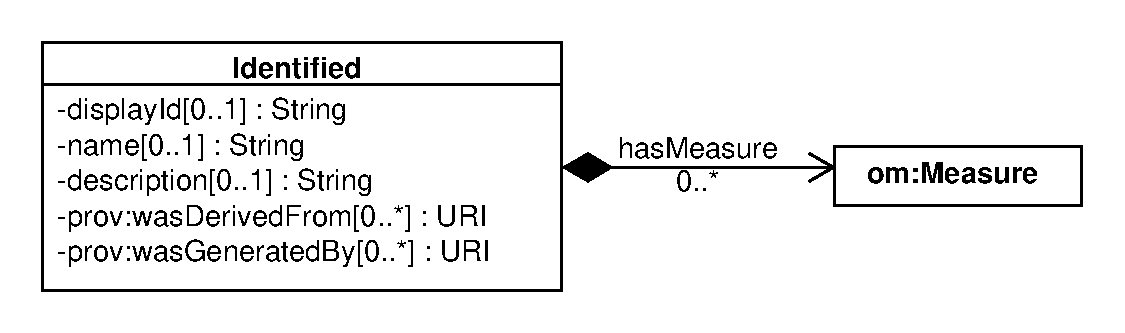
\includegraphics[scale=0.6]{sbol_uml/identified}
\caption[]{Diagram of the \sbol{Identified} abstract class and its associated properties}
\label{uml:identified}
\end{center}
\end{figure}

\begin{itemize}
\item \label{sec:sbol:displayId} 
The \sbol{displayId} property is an OPTIONAL identifier with a data type of \opil{string} (and REQUIRED for objects with URL identifiers). This property is intended to be an intermediate between a URI and the \sbol{name} property that is machine-readable, but more human-readable than the full URI of an object.
If set, its \opil{string} value MUST be composed of only alphanumeric or underscore characters and MUST NOT begin with a digit.

\item \label{sec:sbol:name}
The \sbol{name} property is OPTIONAL and has a data type of \opil{string}. This property is intended to be displayed to a human when visualizing an \sbol{Identified} object.
If an \sbol{Identified} object lacks a name, then software tools SHOULD instead display the object's \sbol{displayId} or URI.

\item \label{sec:sbol:description}
The \sbol{description} property is OPTIONAL and has a data type of \opil{string}. This property is intended to contain a more thorough text description of an \sbol{Identified} object.

\item \label{sec:prov:wasDerivedFrom}
The \prov{wasDerivedFrom} property MAY contain any number of \opil{URI}s. This property is defined by the PROV-O ontology and is located in the \url{https://www.w3.org/ns/prov#} namespace.

\item \label{sec:prov:wasGeneratedBy}
The \prov{wasGeneratedBy} property MAY contain any number of \opil{URI}s. This property is defined by the PROV-O ontology and is located in the \url{https://www.w3.org/ns/prov#} namespace.

\item \label{sec:sbol:hasMeasure}
The \sbol{hasMeasure} property MAY contain any number of \opil{URI}s, each of which refers to a \om{Measure} object that describes a measured parameter for this object.
\end{itemize}

\subsubsection{sbol:TopLevel}
\label{sec:sbol:TopLevel}

\sbol{TopLevel} is an abstract class that is extended by any \sbol{Identified} class that can be found at the top level of an OPIL or SBOL document or file.
In other words, \sbol{TopLevel} objects are never nested inside of any other object as a child object.
The \sbol{TopLevel} classes defined in OPIL are \opil{ProtocolInterface} and \opil{ExperimentRequest}. 

\begin{figure}[ht]
\begin{center}
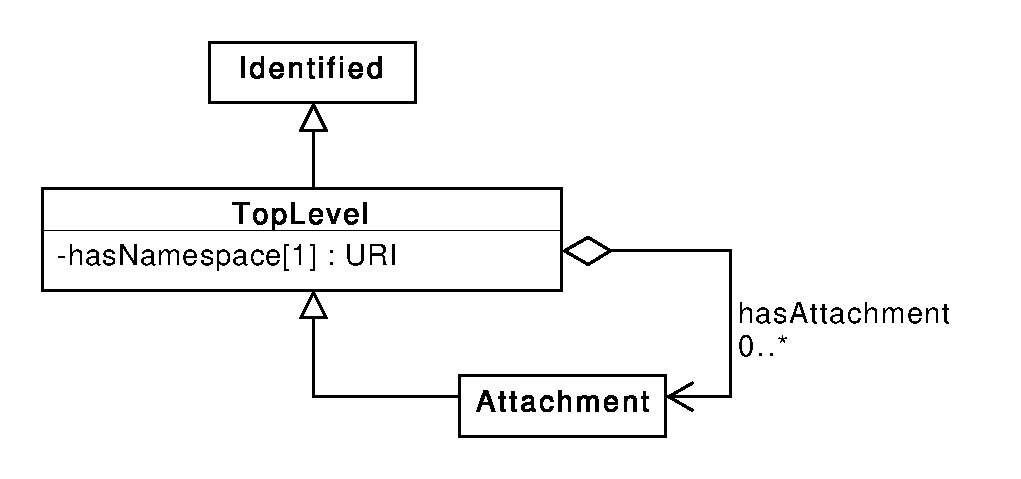
\includegraphics[scale=0.6]{sbol_uml/toplevel}
\caption[]{Classes that inherit from the \sbol{TopLevel} abstract class.}
\label{uml:toplevel}
\end{center}
\end{figure}

\begin{itemize}
\item \label{sec:sbol:hasNamespace}
The \sbol{hasNamespace} property is REQUIRED and MUST contain a single \opil{URI} that defines the namespace portion of URLs for this object and any child objects.
If the URI for the \sbol{TopLevel} object is a URL, then the URI of the \sbol{hasNamespace} property MUST prefix match that URL.

\item 
\label{sec:sbol:hasAttachment}
The \sbol{hasAttachment} property MAY have any number of \opil{URI}s, each referring to an \sbol{Attachment} object.
\end{itemize}


\subsubsection{sbol:Component}
\label{sec:sbol:Component}

The \sbol{Component} class represents the structural and/or functional entities of a biological design. 
In OPIL, this is primarily used to represent the design of experimental samples as combinations of entities such as strains, genetic constructs, media, inducers, etc.

As shown in \ref{uml:component}, the \sbol{Component} class describes a design entity using a number of different properties.
In many OPIL usages, however, the only properties required will be \sbolmult{type:C}{type} and \sbol{hasFeature}.

\begin{figure}[ht]
\begin{center}
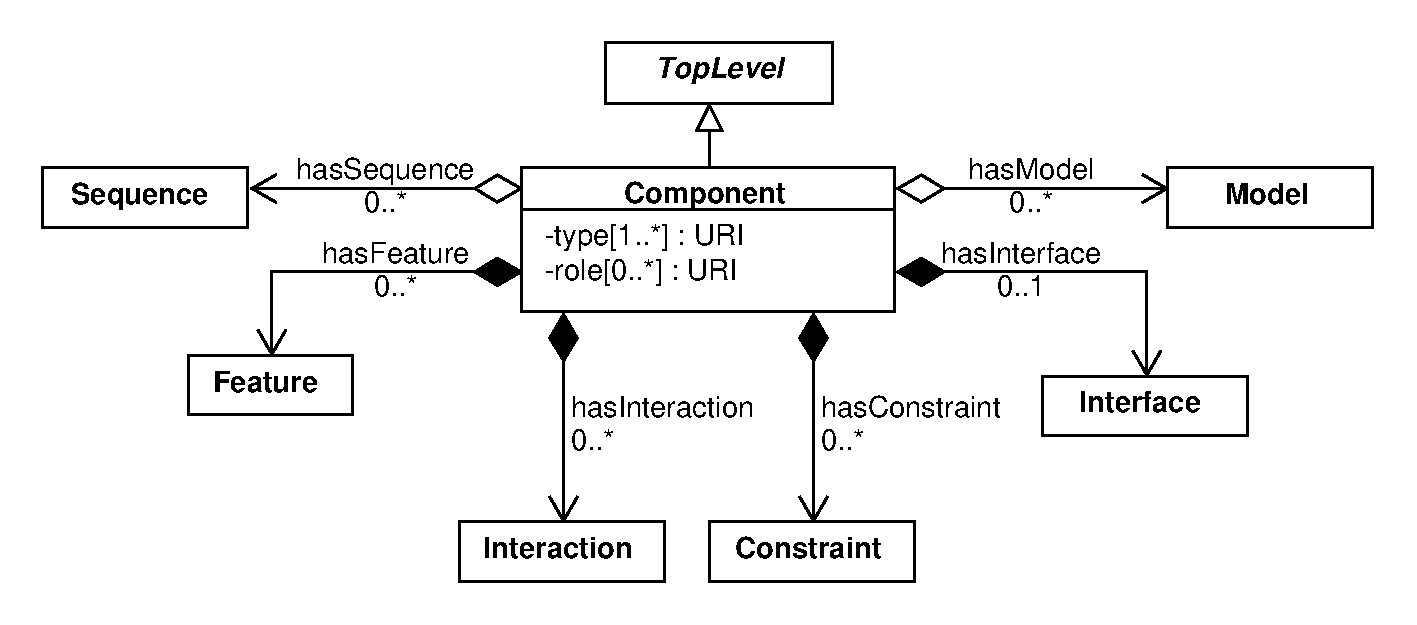
\includegraphics[scale=0.6]{sbol_uml/component}
\caption[]{Diagram of the \sbol{Component} class and its associated properties.}
\label{uml:component}
\end{center}
\end{figure} 

\begin{itemize}
\item \label{sec:sbol:type:C}
The \sbolmult{type:C}{type} property MUST have one or more \opil{URI}s specifying the category of biochemical or physical entity (for example DNA, protein, or simple chemical) that a \sbol{Component} object represents.
For OPIL, this SHOULD be from the physical entity representation branch of the Systems Biology Ontology~\citep{SBO}
and will typically be Functional Entity (\url{https://identifiers.org/SBO:0000241}), which is used to systems of multiple interacting molecules.

\item \label{sec:sbol:hasFeature}
The \sbol{hasFeature} property MAY have any number of \opil{URI}s, each referencing a \sbol{Feature} object. Each \sbol{Feature} represents a specific occurrence of a part, subsystem, or other notable aspect within that design, such as an ingredient in the composition of a growth medium.

\item \label{sec:sbol:role:C}
The \sbolmult{role:C}{role} property MAY have any number of \opil{URI}s, which MUST identify terms from ontologies that are consistent with the \sbolmult{type:C}{type} property of the \sbol{Component}.  
{\em This is not typically required for specifying experimental sample designs in OPIL.}

\item \label{sec:sbol:hasSequence:C}
The \sbolmult{hasSequence:C}{hasSequence} property MAY have any number of \opil{URI}s, each referencing a \sbol{Sequence} object (see \ref{sec:Sequence}).  These objects define the primary structure or structures of the \sbol{Component}.
{\em This is not typically required for specifying experimental sample designs in OPIL.}

\item \label{sec:sbol:hasConstraint}
The \sbol{hasConstraint} property MAY have any number of \opil{URI}s, each referencing a \sbol{Constraint} object.
These objects describe, among other things, any restrictions on the relative, sequence-based positions and/or orientations of the \sbol{Feature} objects contained by the \sbol{Component}, as well as spatial relations such as containment and identity relations.
{\em This is not typically required for specifying experimental sample designs in OPIL.}

\item \label{sec:sbol:hasInteraction}
The \sbol{hasInteraction} property MAY have any number of \opil{URI}s, each referencing an \sbol{Interaction} object describing a behavioral relationship between \sbol{Feature}s in the \sbol{Component}.
{\em This is not typically required for specifying experimental sample designs in OPIL.}

\item \label{sec:sbol:hasInterface}
The \sbol{hasInterface} property is OPTIONAL and MAY have a \opil{URI} referencing an \sbol{Interface} object that indicates the inputs, outputs, and non-directional points of connection to a \sbol{Component}.
{\em This is not typically required for specifying experimental sample designs in OPIL.}

\item \label{sec:sbol:hasModel}
The \sbol{hasModel} property MAY have any number of \opil{URI}s, each referencing a \sbol{Model} object that links the \sbol{Component} to a computational model in any format.
{\em This is not typically required for specifying experimental sample designs in OPIL.}
\end{itemize}

%
%
%\subsubsection{Feature}
%
%\subsubsection{Feature}
%\label{sec:Feature}
%
%The \sbol{Feature} class, as shown in \ref{uml:subcomponent} is used to compose \sbol{Component} objects into a structural or functional hierarchy. 
%
%\begin{figure}[ht]
%\begin{center}
%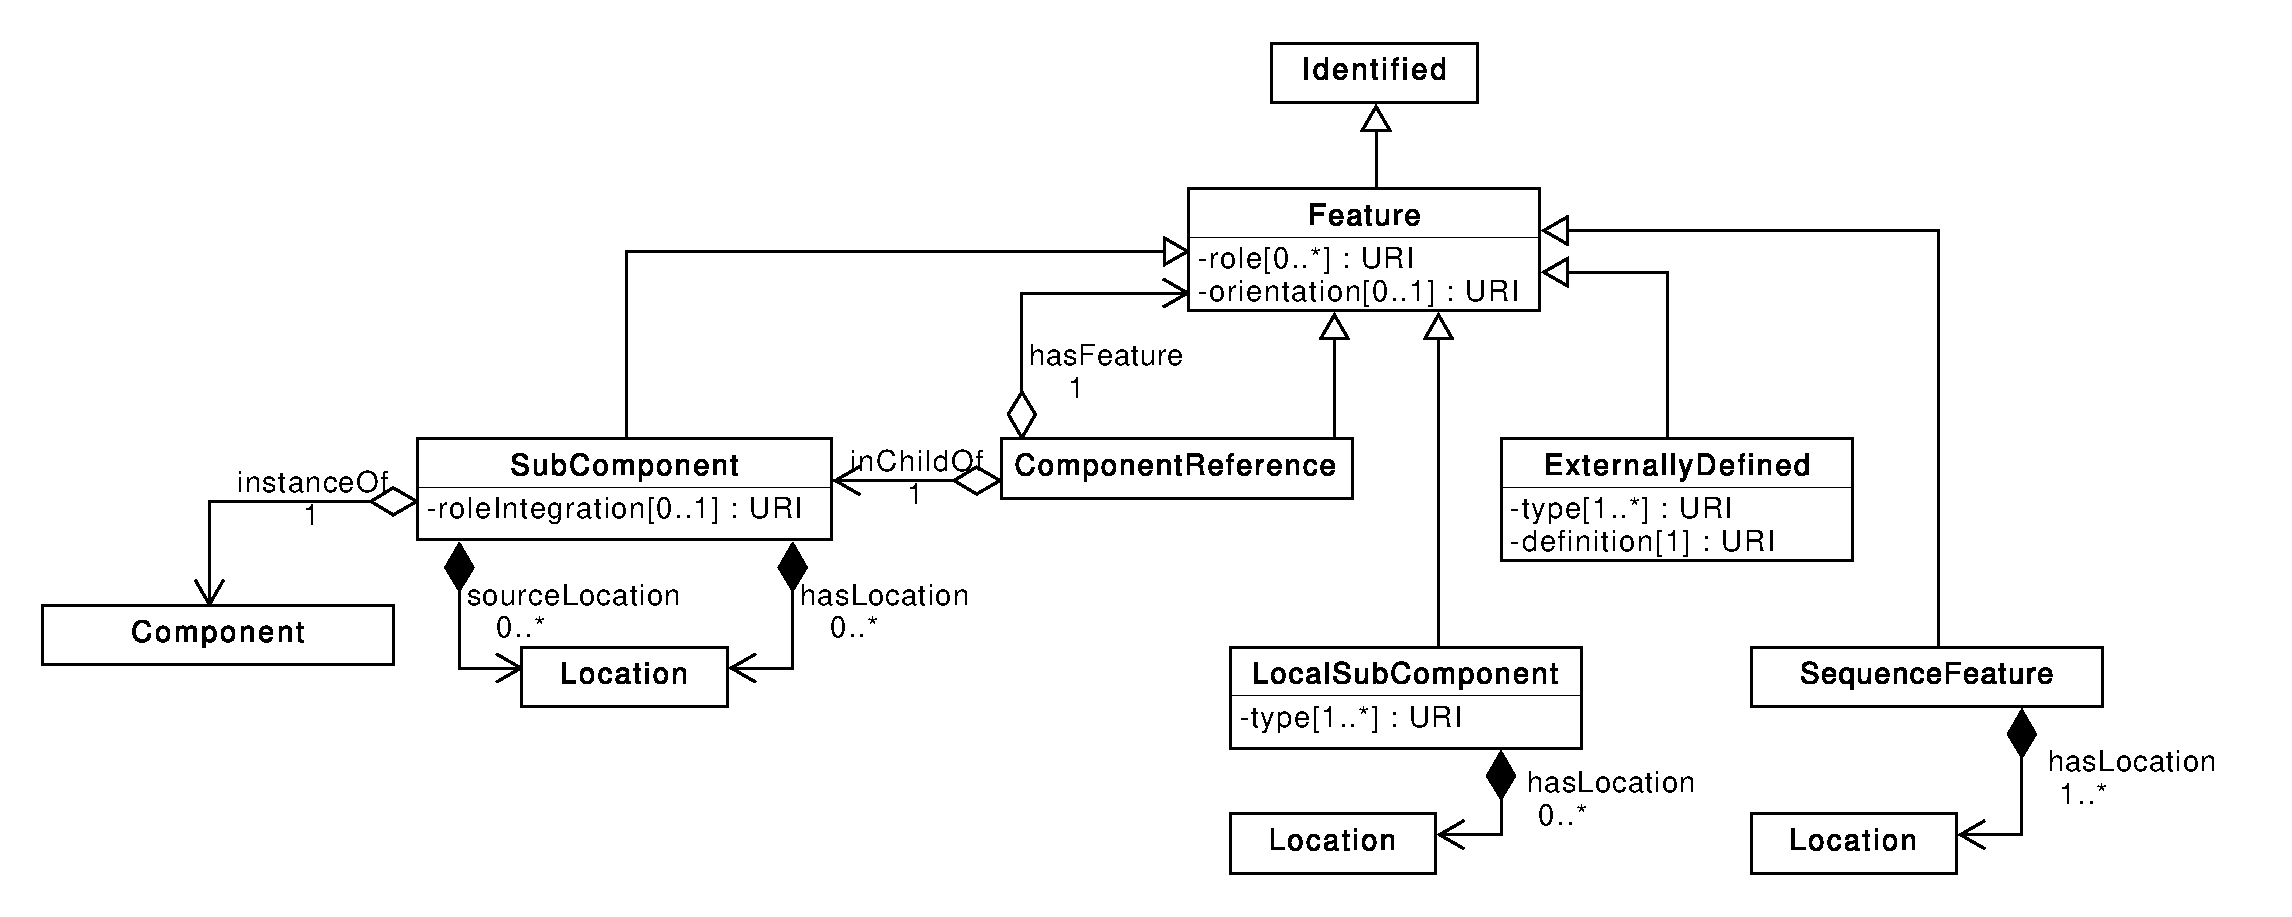
\includegraphics[width=\textwidth]{uml/feature}
%\caption[]{Diagram of the \sbol{Feature} class, its children, and associated properties.}
%\label{uml:subcomponent}
%\end{center}
%\end{figure}
%
%\subparagraph{The \sbolheading{role} property}\label{sec:role:F}
%
%Each \sbol{Feature} can have zero or more \sbolmult{role:F}{role} property \sbol{URI}s describing the purpose or potential function of this \sbol{Feature} in the \textit{context} of its parent \sbol{Component}.
%If the \sbolmult{role:F}{role} for a \sbol{SubComponent} is left unspecified, then the \sbolmult{role:F}{role} is determined by the \sbolmult{role:C}{role} property of the \sbol{Component} that it is an \sbol{instanceOf}. 
%If provided, these \sbolmult{role:F}{role} property \sbol{URI}s MUST identify terms from appropriate ontologies. Roles are not restricted to describing biological function; they may annotate a \sbol{Feature}'s function in any domain for which an ontology exists.
%A table of recommended ontology terms for \sbolmult{role:F}{role} is given in \ref{tbl:component_roles}.
%
%It is RECOMMENDED that these \sbolmult{role:F}{role} property \sbol{URI}s identify terms that are compatible with the \sbolmult{type:C}{type} properties of the \sbol{Feature}'s parent \sbol{Component}.
%For example, a \sbolmult{role:F}{role} of a \sbol{Feature} which belongs to a \sbol{Component} of type DNA might refer to terms from the Sequence Ontology. 
%Likewise, for any feature that is a \sbol{SubComponent}, the \sbolmult{role:F}{role} SHOULD be compatible with the \sbolmult{type:C}{type} of the \sbol{Component} that it links to through its \sbol{instanceOf} property.
%
%\subparagraph{The \sbolheading{orientation} property}
%\label{sec:orientation:F}
%The \sbolmult{orientation:F}{orientation} property is OPTIONAL and has a data type of \sbol{URI}. This can be used to indicate how any associated double-stranded \sbol{Feature} is oriented on the \sbol{elements} of a \sbol{Sequence} from their parent \sbol{Component}. \ref{tbl:orientation_types} provides a list of REQUIRED \sbolmult{orientation:F}{orientation} \sbol{URI}s. If a \sbol{Feature} object has an \sbolmult{orientation:F}{orientation}, then it MUST come from \ref{tbl:orientation_types}.
% 
%
%\begin{table}[ht]
%  \begin{edtable}{tabular}{lp{3.75in}}
%    \toprule
%    \textbf{Orientation URI} & \textbf{Description} \\
%    \midrule
%    \url{http://sbols.org/v3\#inline} & The region specified by this \sbol{Feature} or \sbol{Location} is on the \sbol{elements} of a \sbol{Sequence}. \\
%    \url{http://sbols.org/v3\#reverseComplement} & The region specified by this \sbol{Feature} or \sbol{Location} is on the reverse-complement mapping of the \sbol{elements} of a \sbol{Sequence}. The exact nature of this mapping depends on the \sbol{encoding} of the \sbol{Sequence}. \\
%    \bottomrule
%  \end{edtable}
%  \caption{REQUIRED \sbol{URI}s for the \sbolmult{orientation:F}{orientation} property}
%  \label{tbl:orientation_types}
%\end{table}
%
%\paragraph{SubComponent}
%\label{sec:SubComponent}
%
%The \sbol{SubComponent} class is a subclass of the \sbol{Feature} class that can be used to specify structural hierarchy.
%For example, the \sbol{Component} of a gene might contain four \sbol{SubComponent} objects: a promoter, RBS, CDS, and terminator, each linked to a \sbol{Component} that provides the complete definition.
%In turn, the \sbol{Component} of the promoter \sbol{SubComponent} might itself contain \sbol{SubComponent} objects defining various operator sites, etc.
%
%\subparagraph{The \sbolheading{roleIntegration} property}\label{sec:roleIntegration}
%
%A \sbol{roleIntegration} specifies the relationship between a \sbol{SubComponent} instance's own set of \sbolmult{role:F}{role} properties and the set of \sbolmult{role:C}{role} properties on the included \sbol{Component}.
%
%The \sbol{roleIntegration} property has a data type of \sbol{URI}. A \sbol{SubComponent} instance with zero \sbolmult{role:F}{role} properties MAY OPTIONALLY specify a \sbol{roleIntegration}. A \sbol{SubComponent} instance with one or more \sbolmult{role:F}{role} properties MUST specify a \sbol{roleIntegration} from \ref{tbl:component_roleIntegration}.
%If zero \sbol{SubComponent} \sbolmult{role:F}{role} properties are given and no \sbol{SubComponent} \sbol{roleIntegration} is given, then \url{http://sbols.org/v3\#mergeRoles} is assumed.
%It is RECOMMENDED to specify \sbol{SubComponent} \sbolmult{role:F}{role} values only if the result would differ from the  \sbolmult{role:C}{role} values belonging to this \sbol{SubComponent}'s included \sbol{Component}.
%
%\begin{table}[ht]
%  \begin{edtable}{tabular}{lp{4in}}
%    \toprule
%    \textbf{roleIntegration URI} & \textbf{Description} \\
%    \midrule
%    \url{http://sbols.org/v3\#overrideRoles} & In the context of this \sbol{SubComponent}, ignore any \sbolmult{role:C}{role} given for the included \sbol{Component}. Instead use only the set of zero or more \sbolmult{role:F}{role} properties given for this \sbol{SubComponent}. \\
%    \url{http://sbols.org/v3\#mergeRoles} & Use the union of the two sets: both the set of zero or more \sbolmult{role:F}{role} properties given for this \sbol{SubComponent} as well as the set of zero or more \sbolmult{role:C}{role} properties given for the included \sbol{Component}. \\
%    \bottomrule
%  \end{edtable}
%  \caption{Each \sbol{roleIntegration} mode is associated with a rule governing how a \sbol{SubComponent}'s \sbolmult{role:F}{role} values are to be combined with the included \sbol{Component}'s \sbolmult{role:C}{role} values.}
%  \label{tbl:component_roleIntegration}
%\end{table}
%
%\subparagraph{The \sbolheading{instanceOf} property}
%\label{sec:instanceOf}
%
%The \sbol{instanceOf} property is a REQUIRED \sbol{URI} that refers to the \sbol{Component} providing the definition for this \sbol{SubComponent}.
%Among other things, as described in the previous section, this \sbol{Component} effectively provides information about the \sbolmult{type:C}{type} and \sbolmult{role:C}{role} of the \sbol{SubComponent}.
%
%The \sbol{instanceOf} property MUST NOT refer to the same \sbol{Component} as the one that contains the \sbol{SubComponent}.
%Furthermore, \sbol{SubComponent} objects MUST NOT form a cyclical chain of references via their \sbol{instanceOf} properties and the \sbol{Component} objects that contain them.
%For example, consider the \sbol{SubComponent} objects $A$ and $B$ and the \sbol{Component} objects $X$ and $Y$. The reference chain ``$X$ has feature $A$, $A$ is an instance of $Y$, $Y$ has feature $B$, and $B$ is an instance of $X$'' is cyclical.
%
%
%\subparagraph{The \sbolheading{hasLocation} property}\label{sec:hasLocation:SC}
%
%A \sbol{SubComponent} MAY have any number of \sbolmult{hasLocation:SC}{hasLocation} properties, each of type \sbol{URI}, that MUST refer to \sbol{Location} objects that indicates the location of the \sbol{Sequence} from the \sbol{instanceOf} \sbol{Component} in a \sbol{Sequence} of the parent \sbol{Component}.
%
%If any \sbolmult{hasLocation:SC}{hasLocation} is defined, then there MUST BE precisely one \sbol{Sequence} in the \sbol{instanceOf} \sbol{Component}, as otherwise this relationship is ill-defined.
%
%If no \sbolmult{hasLocation:SC}{hasLocation} is defined, this indicates a part / sub-part relationship for which sequence details have not (yet) been determined or involving types for which sequence relationships are not relevant (e.g., inclusion of a reaction chain within a larger metabolic network).
%
%Allowing multiple \sbol{Location} objects on a single \sbol{SubComponent} is intended to enable representation of discontinuous regions (for example, a coding sequence encoded across a set of exons with interspersed introns).
%As such, the \sbol{Location} objects of a single \sbol{SubComponent} MUST NOT specify overlapping regions, since it is not clear what this would mean.
%There is no such concern with different objects, however, which can freely overlap in \sbol{Location} (for example, specifying overlapping linkers for sequence assembly).
%
%
%\subparagraph{The \sbolheading{sourceLocation} property}\label{sec:sourceLocation}
%
%The \sbol{sourceLocation} property allows for only a portion of a \sbol{Component}'s \sbol{Sequence} to be included, rather than its entirety.
%For example, when composing parts with certain assembly methods, some bases on the boundary may be removed or replaced.
%Another example is describing a deletion or replacement of a portion of a sequence.
%
%A \sbol{SubComponent} MAY have any number of \sbol{sourceLocation} properties, each of type \sbol{URI}, that MUST refer to  \sbol{Location} objects that indicate which \sbol{elements} of the \sbol{instanceOf} \sbol{Component}'s \sbol{Sequence} are used in defining the parent of the \sbol{SubComponent}.
%
%If there are no \sbol{sourceLocation} properties, then the whole \sbol{Sequence} is assumed to be included. 
%
%
%\paragraph{ComponentReference}
%\label{sec:ComponentReference}
%
%The \sbol{ComponentReference} class is a subclass of \sbol{Feature} that can be used to reference \sbol{Feature}s within\\ \sbol{SubComponent}s. 
%
%\subparagraph{The \sbolheading{inChildOf} property}\label{sec:inChildOf}
%
%The \sbol{inChildOf} property is a REQUIRED \sbol{URI} that refers to a \sbol{SubComponent}. 
%The \sbol{inChildOf} property MUST refer to a \sbol{SubComponent} pointed directly to by the parent of the \sbol{ComponentReference}.
%Specifically:
%\begin{itemize}
%\item If the parent of the \sbol{ComponentReference} is a \sbol{Component}, then \sbol{inChildOf} MUST be one of its \sbol{SubComponent}s.
%\item If the parent of the \sbol{ComponentReference} is another \sbol{ComponentReference}, then \sbol{inChildOf} MUST be a \sbol{SubComponent} of the \sbol{Component} linked as \sbol{instanceOf} the parent's \sbol{inChildOf} \sbol{SubComponent}.
%\end{itemize}
%
%\subparagraph{The \sbolheading{hasFeature} property}\label{sec:hasFeature:CR}
%
%The \sbolmult{hasFeature:CR}{hasFeature} property is a REQUIRED \sbol{URI} that refers to a \sbol{Feature}.
%
%This can be used to either link to the \sbol{Feature} being referenced or to chain hierarchically through additional layers of \sbol{SubComponent}.
%\begin{itemize}
%\item If the \sbol{Feature} is a \sbol{ComponentReference}, then that \sbol{ComponentReference} acts as a hierarchical link in a chain of references, and MUST be either a child of the \sbol{ComponentReference} linking to it via \sbolmult{hasFeature:CR}{hasFeature} or a child of the \sbol{Component} linked as \sbol{instanceOf} the \sbol{ComponentReference}'s \sbol{inChildOf} \sbol{SubComponent}.
%\item Otherwise, if the \sbol{hasFeature} refers to any other type of \sbol{Feature}, that \sbol{Feature} MUST be a child of the \sbol{Component} linked as \sbol{instanceOf} the \sbol{ComponentReference}'s \sbol{inChildOf} \sbol{SubComponent}.
%\end{itemize}
%
%For example, \sbol{ComponentReference} R1 looking into a \sbol{SubComponent} for a plasmid might link with \sbol{hasFeature} to its own child \sbol{ComponentReference} R2, which in turn looks within the \sbol{Component} defining the plasmid to the plasmid's CDS \sbol{SubComponent}, in turn using \sbol{hasFeature} to reference a \sbol{SequenceFeature} within the \sbol{Component} that defines that CDS.
%
%\paragraph{LocalSubComponent}
%\label{sec:LocalSubComponent}
%
%The \sbol{LocalSubComponent} class is a subclass of \sbol{Feature}. 
%This class serves as a way to create a placeholder in more complex \sbol{Component}s, such as a variable to be filled in later or a composite that exists only within the context of the parent \sbol{Component}.
%
%\subparagraph{The \sbolheading{type} property}\label{sec:type:LSC}
%
%The \sbolmult{type:LSC}{type} property is REQUIRED and contains one or more \sbol{URI}s. The \sbolmult{type:LSC}{type} property is identical to its use in \sbol{Component}.
%
%\subparagraph{The \sbolheading{hasLocation} property}\label{sec:hasLocation:LSC}
%
%A \sbol{LocalSubComponent} MAY have any number of \sbolmult{hasLocation:LSC}{hasLocation} properties, each of type \sbol{URI}, that MUST refer to \sbol{Location} objects. 
%These follow the same restrictions as for the \sbolmult{hasLocation:SC}{hasLocation} of a \sbol{SubComponent}, notably that the \sbol{Location}s of \sbolmult{hasLocation:LSC}{hasLocation} properties attached to the same \sbol{LocalSubComponent} MUST NOT overlap.
%
%\paragraph{ExternallyDefined}
%\label{sec:ExternallyDefined}
%
%The \sbol{ExternallyDefined} class has been introduced so that external definitions in databases like ChEBI or UniProt can be referenced.
%
%\subparagraph{The \sbolheading{type} property}\label{sec:type:ED}
%
%The \sbolmult{type:ED}{type} property is REQUIRED and contains one or more \sbol{URI}s. The \sbolmult{type:ED}{type} property is identical to its use in \sbol{Component}.
%
%\subparagraph{The \sbolheading{definition} property}\label{sec:definition:ED}
%
%The \sbolmult{definition:ED}{definition} property is REQUIRED and is of type \sbol{URI} that links to a canonical definition external to SBOL.
%When possible, such definitions SHOULD use the recommended external resources in \ref{sec:recomm_ontologies}.
%For example, an \sbol{ExternallyDefined} simple chemical might link to ChEBI and a protein might link to UniProt.
%
%\paragraph{SequenceFeature}
%\label{sec:SequenceFeature}
%
%The \sbol{SequenceFeature} class describes one or more regions of interest on the \sbol{Sequence} objects referred to by its parent \sbol{Component}. 
%
%\subparagraph{The \sbolheading{hasLocation} property}\label{sec:hasLocation:SF}
%
%\threezeroone{The \sbolmult{hasLocation:SF}{hasLocation} is REQUIRED and contains one or more \sbol{URI}s, which} MUST refer to \sbol{Location} objects. 
%These follow the same restrictions as for the \sbolmult{hasLocation:SC}{hasLocation} of a \sbol{SubComponent}, notably that the \sbol{Location}s of \sbolmult{hasLocation:SF}{hasLocation} properties attached to the same \sbol{SequenceFeature} MUST NOT overlap.
%
%
%\subsubsection{CombinatorialDerivation}
%
%\subsection{CombinatorialDerivation}
%\label{sec:CombinatorialDerivation}
%
%The purpose of the \sbol{CombinatorialDerivation} class is to specify combinatorial biological designs without having to specify every possible design variant. For example, a \sbol{CombinatorialDerivation} can be used to specify a library of reporter gene variants that include different promoters and RBSs without having to specify a \sbol{Component} for every possible combination of promoter, RBS, and CDS in the library. \sbol{Component} objects that realize a \sbol{CombinatorialDerivation} can be derived in accordance with the class properties \sbol{template}, \\
%\threezeroone{\st{hasVariableComponent}} \threezeroone{\sbol{hasVariableFeature}}, and \sbol{strategy} (see \ref{uml:combinatorial_derivation}).
%
%\begin{figure}[ht]
%\begin{center}
%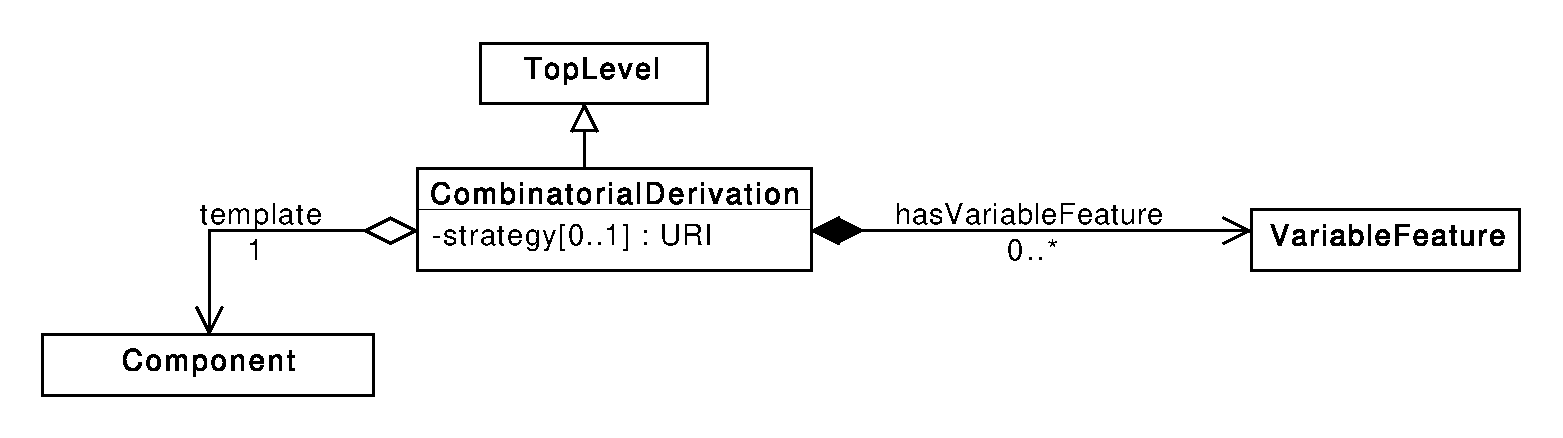
\includegraphics[scale=0.6]{uml/combinatorial_derivation}
%\caption[]{Diagram of the \sbol{CombinatorialDerivation} class and its associated properties.}
%\label{uml:combinatorial_derivation}
%\end{center}
%\end{figure}
%
%\subparagraph{The \sbolheading{template} property}\label{sec:template}
%
%The \sbol{template} property is REQUIRED and MUST contain a URI that refers to a \sbol{Component}. 
%This \sbol{Component} is expected to serve as a template for the derivation of new \sbol{Component} objects. 
%Consequently, its \sbol{hasFeature} properties SHOULD contain one or more \threezeroone{\st{SubComponent objects that describe its substructure (referred to hereafter as template SubComponent objects), and its hasConstraint property MAY also contain one or more Constraint objects that constrain this substructure}} \threezeroone{\sbol{Feature} objects that describe its substructure (referred to hereafter as template \sbol{Feature} objects), and its other properties MAY also describe other aspects of the template that will not change based on the values that ay be varied.}
%
%When a \sbol{Component} is derived in accordance with a \sbol{CombinatorialDerivation}, the \prov{wasDerivedFrom} property of the derived \sbol{Component} SHOULD refer to the \sbol{CombinatorialDerivation}. When multiple \sbol{Component} objects are derived in accordance with the same \sbol{CombinatorialDerivation}, they MAY be referred to by the \sbol{member} property of a \sbol{Collection}, in which case the \prov{wasDerivedFrom} property of the \sbol{Collection} SHOULD also refer to this \sbol{CombinatorialDerivation}.
%
%If the \sbolmult{type:C}{type} property of the template \sbol{Component} contains one or more URIs, then the \sbolmult{type:C}{type} property of any derived \sbol{Component} SHOULD also contain those URIs. 
%The same holds true for the \sbolmult{role:C}{role} properties of these \sbol{Component} objects.
%
%\threezeroone{\st{The hasVariableComponent property}}
%\threezeroone{\subparagraph{The \sbolheading{hasVariableFeature} property}}\label{sec:hasVariableFeature}
%
%Each \threezeroone{\st{VariableComponent}} \threezeroone{\sbol{VariableFeature}} child of a \sbol{CombinatorialDerivation} defines the set of possible values for one of the variables in the \sbol{template}.
%A \sbol{CombinatorialDerivation} object can have zero or more \threezeroone{\st{hasVariableComponent}} \sbol{hasVariableFeature} properties, each of type \sbol{URI}, specifying a \threezeroone{\st{hasVariableComponent}} \sbol{VariableFeature}. 
%The set of \threezeroone{\st{hasVariableComponent}} \sbol{hasVariableFeature} properties MUST NOT contain two or more \threezeroone{\st{variableComponent}} \sbol{VariableFeature} objects that refer to the same template \threezeroone{\st{SubComponent}} \sbol{Feature} via their \sbol{variable} properties (i.e., do not define the same variable twice).
%
%The \sbol{variable} properties of \threezeroone{\st{VariableComponent}} \sbol{VariableFeature} objects control which \threezeroone{\st{SubComponent}} \sbol{Feature} objects in the \sbol{template} are modified in a derived \sbol{Component}.
%If no \sbol{variable} property of one of these \threezeroone{\st{VariableComponent}} \sbol{VariableFeature} objects refers to a template \threezeroone{\st{SubComponent}} \sbol{Feature}, then it is not a variable and the derived object SHOULD have a \threezeroone{\st{SubeComponent}} \sbol{Feature} with identical properties
%and a \prov{wasDerivedFrom} property that refers to the template \threezeroone{\st{SubComponent}} \sbol{Feature}.
%
%If a \threezeroone{\st{SubComponent}} \sbol{Feature} in the \sbol{template} is referred to by some \sbol{variable} in a \threezeroone{\st{VariableComponent}} \sbol{VariableFeature}, then it is a variable and it SHOULD be replaced in the derived \sbol{Component} by a number of \threezeroone{\st{SubComponent}} \sbol{Feature} objects constrained by the number specified by the \sbol{cardinality} property of the \threezeroone{\st{VariableComponent}} \sbol{VariableFeature} (see \ref{tbl:cardinality}).
%Each \threezeroone{\st{instanceOf property of such a SubComponent object in the derived Component MUST refer to a Component object specified by a variant, contained within a variantCollection, or derived from a variantDerivation of the VariableComponent}} \threezeroone{property of such a \sbol{Feature} object in the derived \sbol{Component} MUST be derived from the values of the  associated \sbol{VariableFeature}}.
%
%
%Finally, all derived \threezeroone{\st{SubComponent}} \sbol{Feature} objects MUST follow the \sbol{restriction} properties of any 
%\sbol{Constraint} objects that refer to their corresponding template \threezeroone{\st{SubComponent}} \sbol{Feature}, and SHOULD have values of \sbolmult{role:F}{role} that contain the same values as the \sbolmult{role:F}{role} in the template \threezeroone{\st{SubComponent}} \sbol{Feature}.
%
%
%\subparagraph{The \sbolheading{strategy} property}\label{sec:strategy}
%The \sbol{strategy} property is OPTIONAL and has a data type of URI. \ref{tbl:strategy} provides a list of REQUIRED \sbol{strategy} URIs. If the \sbol{strategy} property is not empty, then it MUST contain a URI from \ref{tbl:strategy}. This property recommends how many \sbol{Component} objects SHOULD be derived from the template \sbol{Component}.
%
%\begin{table}[ht]
%  \begin{edtable}{tabular}{lp{4in}}
%    \toprule
%    \textbf{Strategy URI} & \textbf{Description} \\
%    \midrule
%    \url{http://sbols.org/v3#enumerate}  &  Derivation SHOULD produce all possible \sbol{Component} objects specified by the \sbol{CombinatorialDerivation}. \\
%        \url{http://sbols.org/v3#sample}  & Derivation SHOULD produce a subset of possible \sbol{Component} objects specified by \sbol{CombinatorialDerivation}. The manner in which this subset is chosen is left unspecified. \\
%    \bottomrule
%  \end{edtable}
%  \caption{REQUIRED \sbol{URI}s for the \sbol{strategy} property.}
%  \label{tbl:strategy}
%\end{table}
%
%\subsubsection{VariableFeature}
%\label{sec:VariableFeature}
%
%As described \sbolmult{hasVariableFeature}{above}, the \threezeroone{\st{VariableComponent}} \sbol{VariableFeature} class specifies a variable and set of values that will replace one of the \threezeroone{\st{SubComponent}} \sbol{Feature} objects in the \sbol{template} of a \sbol{CombinatorialDerivation}.
%The variable is specified by the \sbol{variable} property,
%and the set of values is defined by the union of \sbol{Component} objects referred to by the \sbol{variant}, \sbol{variantCollection}, and \sbol{variantDerivation} properties.
%
%Note that this union is intended to be a set and not a multi-set.
%For example, if the \sbol{variant} property contains a \sbol{Component} $A$ and the \sbol{variantCollection} property has a \sbol{Collection} containing both \sbol{Component} $A$ and  \sbol{Component} $B$, then $A$ SHOULD NOT be selected twice during enumeration, and it SHOULD NOT be selected twice as much as $B$ during sampling.
%
%\threezeroone{Given a set of values linked from a \sbol{VariableFeature}, it SHOULD be the case that all value are of type \sbol{om:Measure} or else all values are of type \sbol{Feature}. At present, it is explicitly left undefined how derivation of new components ought to handle mixtures of \sbol{om:Measure} and \sbol{Feature} values.}
%
%\begin{figure}[ht]
%\begin{center}
%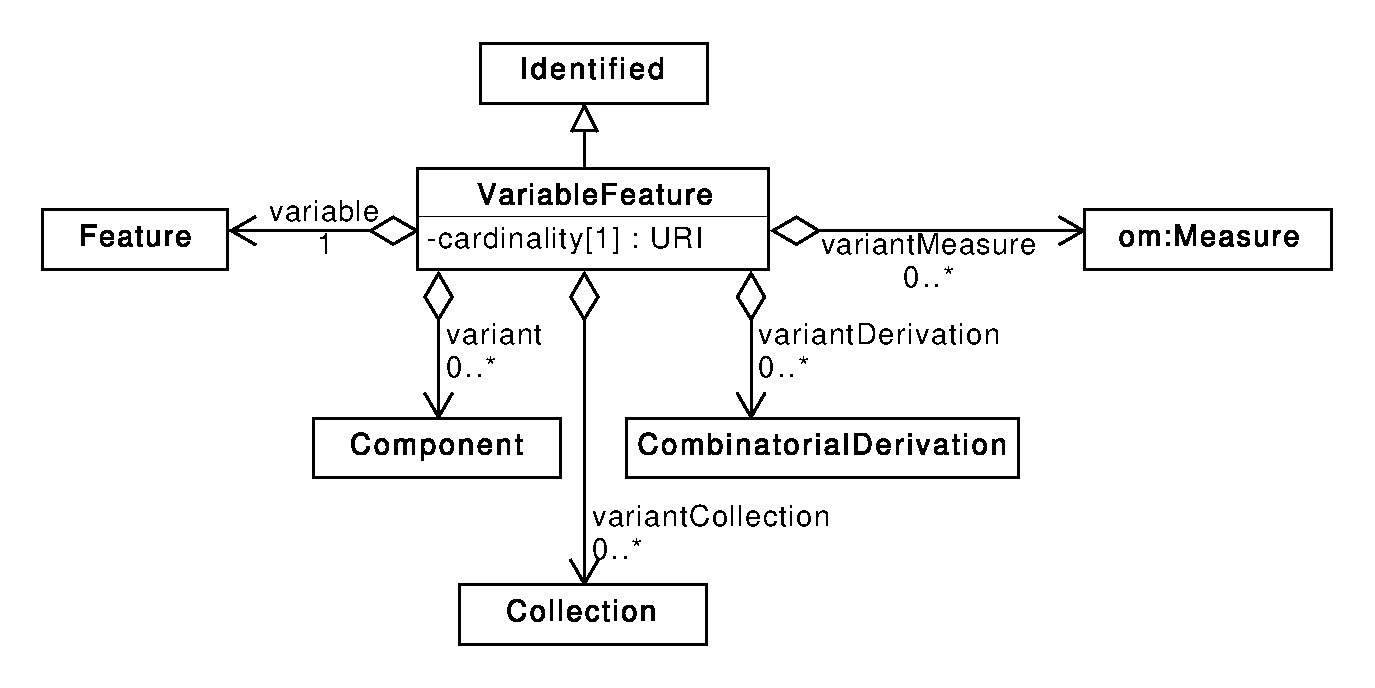
\includegraphics[scale=0.6]{uml/variable_component}
%\caption[]{Diagram of the \sbol{VariableFeature} class and its associated properties.}
%\label{uml:variable_component}
%\end{center}
%\end{figure}
%
%\subparagraph{The \sbolheading{variable} property}\label{sec:variable}
%
%The \sbol{variable} property is REQUIRED and MUST contain a URI that refers to a template \threezeroone{\st{SubComponent}} \sbol{Feature} in the \sbol{template} \sbol{Component} referred to by this \threezeroone{\st{VariableComponent's}} \sbol{VariableFeature}'s parent \sbol{CombinatorialDerivation}
%
%\threezeroone{\subparagraph{The \sbolheading{variantMeasure} property}\label{sec:variantMeasure}
%
%A \threezeroone{\st{VariableComponent}} \sbol{VariableFeature} object can have zero or more \sbol{variantMeasure} properties, each of type \sbol{URI}, specifying a \sbol{om:Measure} object. This property specifies numerical values that are options to be applied to the \sbol{variable} \threezeroone{\st{SubComponent}} \sbol{Feature} from the \sbol{template} when deriving a new \sbol{Component}.
%
%Note that because a \sbol{om:Measure} is not a \sbol{TopLevel}, the vlaues of \sbol{variantMeasure} must be child objects of the \sbol{VariableFeature}.}
%
%\subparagraph{The \sbolheading{variant} property}\label{sec:variant}
%
%A \threezeroone{\st{VariableComponent}} \sbol{VariableFeature} object can have zero or more \sbol{variant} properties, each of type \sbol{URI}, specifying a \sbol{Component} object. This property specifies individual \sbol{Component} objects to serve as options when deriving a new \threezeroone{\st{SubComponent}} \sbol{Feature} for the \sbol{variable} \threezeroone{\st{SubComponent}} \sbol{Feature} from the \sbol{template}.
%
%\subparagraph{The \sbolheading{variantCollection} property}\label{sec:variantCollection}
%
%A \threezeroone{\st{VariableComponent}} \sbol{VariableFeature} object can have zero or more \sbol{variantCollection} properties, each of type \sbol{URI}, specifying a \sbol{Collection} object.
%Such a \sbol{Collection} MUST NOT contain any objects besides \sbol{Component} objects or \sbol{Collection} objects that themselves contain only \sbol{Component} or \sbol{Collection} objects.
%This property enables the specification of existing groups of \sbol{Component} objects to serve as options.
%
%\subparagraph{The \sbolheading{variantDerivation} property}\label{sec:variantDerivation}
%
%A \threezeroone{\st{VariableComponent}} \sbol{VariableFeature} object can have zero or more \sbol{variantDerivation} properties, each of type \sbol{URI}, specifying a \sbol{CombinatorialDerivation} object. 
%This property enables the specification of \sbol{Component} objects derived in accordance with another \sbol{CombinatorialDerivation} to serve as options when deriving a new \threezeroone{\st{SubComponent}} \sbol{Feature} for the \sbol{variable} \threezeroone{\st{SubComponent}} \sbol{Feature} from the \sbol{template}. 
%The \sbol{variantDerivation} properties of a \threezeroone{\st{VariableComponent}} \sbol{VariableFeature} MUST NOT refer to the \sbol{CombinatorialDerivation} that contains this \threezeroone{\st{VariableComponent}} \sbol{VariableFeature}. 
%Furthermore, such \threezeroone{\st{VariableComponent}} \sbol{VariableFeature} objects MUST NOT form a cyclical chain of references via their \sbol{variantDerivation} properties and the \sbol{CombinatorialDerivation} objects that contain them. 
%
%\subparagraph{The \sbolheading{cardinality} property}\label{sec:cardinality}
%
%The \sbol{cardinality} property is REQUIRED and has type of URI. This property specifies how many \threezeroone{\st{SubComponent}} \sbol{Feature} objects SHOULD be derived from the template \threezeroone{\st{SubComponent}} \sbol{Feature} during the derivation of a new \sbol{Component}. The URI value of this property MUST come from the URIs provided in~\ref{tbl:cardinality}.
%
%\begin{table}[ht]
%  \begin{edtable}{tabular}{lp{4in}}
%    \toprule
%    \textbf{Cardinality URI} & \textbf{Description} \\
%    \midrule
%    \url{http://sbols.org/v3#zeroOrOne} & No more than one \sbol{Feature} in the derived \sbol{Component} SHOULD have a \prov{wasDerivedFrom} property that refers to the template \sbol{Feature}. \\
%        \url{http://sbols.org/v3#one} & Exactly one \sbol{Feature} in the derived \sbol{Component} SHOULD have a \prov{wasDerivedFrom} property that refers to the template \sbol{Feature}. \\
%\url{http://sbols.org/v3#zeroOrMore} & Any number of \sbol{Feature} objects in the derived \sbol{Component} MAY have \prov{wasDerivedFrom} properties that refer to the template \sbol{Feature}. \\
%\url{http://sbols.org/v3#oneOrMore} & At least one \sbol{Feature} in the derived \sbol{Component} SHOULD have a \prov{wasDerivedFrom} property that refers to the template \sbol{Feature}. \\
%    \bottomrule
%  \end{edtable}
%  \caption{REQUIRED \sbol{URI}s for the \sbol{cardinality} property.}
%  \label{tbl:cardinality}
%\end{table}
%
%
%\subsubsection{VariableFeature}
%
%

\subsection{Ontology of Units of Measure}

In most cases where a number is needed in OPIL, that number is a measure with units associated with it.
The Ontology of Units of Measure (OM) (\url{http://www.ontology-of-units-of-measure.org/resource/om-2}) already defines a data model for representing measures and their associated units. 
A subset of OM, already adopted by SBOL, is used for this purpose by OPIL as well.

The key class used is \om{Measure}, which associates a number with a unit and a biology-related property.
In most cases, it should be possible to use one of the \om{Unit} instances already defined by OM; when this is not possible, an appropriate unit can be defined using \om{Unit} and \om{Prefix} classes.

\subsubsection{om:Measure} \label{sec:om:Measure}

The purpose of the \om{Measure} class is to link a numerical value to a \om{Unit}. 

\begin{itemize}
\item \label{sec:om:hasNumericalValue}
The \om{hasNumericalValue} property is REQUIRED and MUST contain a single \opil{float}.

\item \label{sec:om:hasUnit:Measure}
The \ommult{hasUnit:Measure}{hasUnit} property is REQUIRED and MUST contain a \opil{URI} that refers to a \om{Unit}. 

\item \label{sec:sbol:type:Measure}
The \sbolmult{type:Measure}{type} property MAY contain any number of \opil{URI}s. It is RECOMMENDED that one of these \opil{URI}s identify a term from the Systems Description Parameter branch of the Systems Biology Ontology (SBO) (\url{http://www.ebi.ac.uk/sbo/main/}). This \sbolmult{type:Measure}{type} property was added by SBOL to describe different types of parameters 
(for example, rate of reaction is identified by the SBO term \url{http://identifiers.org/SBO:0000612}).


\end{itemize}



